\subsection{Ábrák}
	
Ez itt a \ref{fig:ur5} ábra.
\begin{figure}[H]
	\centering
	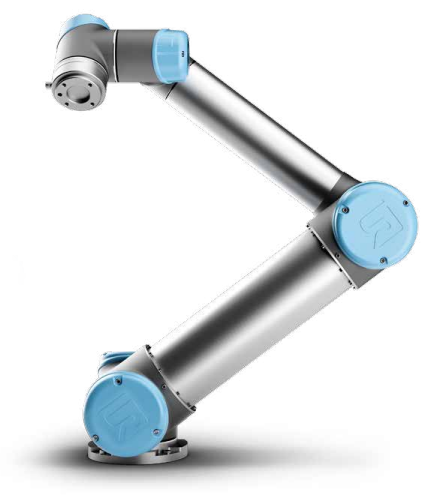
\includegraphics[width=0.5\linewidth]{img/ur5robot.png}
	\caption{UR5 kollaboratív robot}
	\label{fig:ur5}
\end{figure}


\subsection{Hivatkozások}

Ez itt egy folyóirat cikk \cite{journal-example}.

Ez itt egy konferencia cikk \cite{conference-example}.

Ez itt egy könyv \cite{book-example}.

Ez itt egy online forrás \cite{online-example}.

Ez itt egy disszertáció \cite{thesis-example}.

	
\subsection{Táblázatok}
Példaként itt látható egy táblázat \ref{tab:ur5}.

\begin{table}[H]
	\centering
	\begin{tabular}{|c|c|}
	    \hline
		Tulajdonság                      & Érték    \\ \hline
		kinyúlás {[}mm{]}                & 850      \\ \hline
		Szabadságfok                     & 6        \\ \hline
		Teherbírás {[}kg{]}               & 5        \\ \hline
		Súly {[}kg{]}                    & 18,4     \\ \hline
		Ismétlési pontosság {[}mm{]}     & $\pm0,1$    \\ \hline
		Teljesítményfelvétel {[}W{]}     & 90-325   \\ \hline
		Csuklók mozgástartománya {[}$^{\circ}${]} & $\pm360$    \\ \hline
		Max. csuklósebesség {[}$^{\circ}/sec${]}  & $\pm180$    \\ \hline
		Max. Tool sebesség {[}m/s{]}     & 1        \\ \hline
		Programozási nyelv               & URscript \\ \hline
	\end{tabular}
	\caption{Az UR5 robot főbb paraméterei}
	\label{tab:ur5}
\end{table}

Egy másik a \ref{tab:joint-limits} táblázat.

\begin{table}[H]
    \centering
    \begin{tabular}{|c|c|c|c|c|}
        \hline
    	Robotcsukló & \begin{tabular}[c]{@{}c@{}}min. poz.\\ {[}rad{]}\end{tabular} & \begin{tabular}[c]{@{}c@{}}max. poz.\\ {[}rad{]}\end{tabular} & \begin{tabular}[c]{@{}c@{}}max. sebesség\\ {[}rad/s{]}\end{tabular} & \begin{tabular}[c]{@{}c@{}}max. gyorsulás\\ \hline {[}rad/s\textasciicircum{}2{]}\end{tabular} \\ \hline
    	1 & -0.802 & 1.39 & 3.1 & 9 \\ \hline
    	2 & -2.25 & -0.873 & 3.1 & 9 \\ \hline
    	3 & 1.25 & 2.7 & 3.1 & 9 \\ \hline
    	4 & -3.49 & -1.41 & 3.1 & 9 \\ \hline
    	5 & -2.62 & -0.62 & 3.1 & 9 \\ \hline
    	6 & -3.14 & 2.09 & 3.1 & 9 \\ \hline
    \end{tabular}
    \caption{Másik példa táblázat}
    \label{tab:joint-limits}
\end{table}

	
\subsection{Képlet}

Ez itt a \ref{eq:keplet1} képlet:
\begin{align}
    \cos{\alpha-\beta} = \cos{\alpha}\cdot\sin{\beta}-\cos{\beta}\cdot\sin{\alpha}
    \label{eq:keplet1}
\end{align}	

	
\subsection{Felsorolás}

Ez egy felsorolás:
\begin{itemize}
	\item A felsorolás első eleme
	\item A felsorolás második eleme
	\item A felsorolás harmadik eleme
\end{itemize}